%% Single vs multiple ANN paper, draft v0, 2026-11-03 (Spain time).
%% Target: Combustion and Flame (Elsevier, elsarticle); alternative Energy and AI.
%% Sources: docs/ENSEMBLE-ROADMAP.md section 11 and chemmanifold/ensemble/ (e0_deep_ensemble, e1_error_map,
%%   e3/*, e4/pure_ood8, e4/pure_p0). Common elements follow papers/isann-vs-iterml (PR #20).
%% \todo{} = must be resolved before submission. Check every reference in refs.bib against the paper.
\documentclass[preprint,review,12pt]{elsarticle}

\usepackage[T1]{fontenc}
\usepackage{lmodern}
\usepackage{amsmath,amssymb}
\usepackage{graphicx}
\usepackage{booktabs}
\usepackage{siunitx}
\usepackage{lineno}
\usepackage{xcolor}
\usepackage[hidelinks]{hyperref}
\newcommand{\todo}[1]{\textcolor{red}{[TODO: #1]}}
\sisetup{group-separator={\,},group-minimum-digits=4}
\linenumbers
\journal{Combustion and Flame}

\begin{document}
\begin{frontmatter}

\title{One network or several? Deep ensembles and region experts for neural chemistry surrogates in a
laminar methane flame}

\author[a]{Javier \todo{surname}}
\author[a]{\todo{co-authors}}
\address[a]{\todo{affiliation}}

\begin{abstract}
Neural-network surrogates of finite-rate chemistry are usually a single network that maps the
composition at the start of a chemistry step to that at its end. We ask whether a \emph{set} of networks
represents the chemistry better, under three constraints: the training data come only from
physics-based exploration of the thermochemical space with Cantera (no state of the target simulation is
ever a training pair), the set is called through the same chemistry-step interface as one network, and
its cost is measured in the flow solver. Two kinds of set are tested on an 18-species methane mechanism
(GA18): a \emph{deep ensemble} that averages the mass fractions of three networks trained from scratch
with different seeds, and \emph{region experts}, three networks trained on boxes of temperature and
normalised progress variable and blended by a soft gate that reads the input state only. An error map of
the single network shows why a split is tempting: 64\% of its one-step temperature error sits in 2\% of
the data (reacting near-stoichiometric gas at 1200--1900~K). On a fixed offline benchmark of 440
canonical Cantera states, the ensemble's 10~ms temperature error is 15~K against 25--45~K for its three
members, and the members' disagreement after one step predicts the error (Spearman 0.83). Region experts
warm-started from the single network were worse than it, as was a single network fine-tuned in the same
way, while experts trained from scratch were better on average than single networks (29 against 37~K)
but with overlapping seed ranges. In a laminar burner simulation run without any direct-integration
fallback, the ensemble reduced the mean flame-zone temperature error from 24.2 to 4.4~K and brought the
domain totals of CO and OH at 50~ms from 4.4 and 5.5 times to 0.93 and 1.19 times the direct integration, while
keeping 99.6\% of the flame cells inside the trained range, at 2.9 times the cost per step. The ignition
of the fuel jet stayed 0.9~ms early, which averaging cannot correct because all members share the same
training data. Averaging independent networks is a cheap, robust gain; partitioning the space needs more
than a gate to pay off.
\end{abstract}

\begin{keyword}
Chemistry acceleration \sep Neural network surrogate \sep Deep ensemble \sep Mixture of experts \sep
Uncertainty estimation \sep Thermochemical space exploration
\end{keyword}
\end{frontmatter}

%% ===============================================================================================
\section{Introduction}
\label{sec:intro}

The integration of stiff finite-rate chemistry dominates the cost of many reacting-flow simulations, and
artificial neural networks (ANN) have been used to replace the integrator since the
1990s~\cite{christo1996ann,blasco1998ann}. Since the chemistry of a flame covers very different regimes,
from cold mixing to fast radical chemistry in the reaction zone and slow relaxation of the burnt gas,
several authors split the composition space and trained one network per region, for example with
self-organising maps~\cite{chatzopoulos2013rcce,franke2017rcce,ding2021hybrid,readshaw2021hybrid}. The
machine-learning literature offers two other reasons to use more than one network: averaging
independently trained networks (deep ensembles) reduces the variance of the prediction and its spread
estimates the uncertainty~\cite{dietterich2000ensembles,lakshminarayanan2017ensembles}; and a mixture of
experts lets each network specialise where a gate sends it~\cite{jacobs1991moe}.

Whether a set of networks is worth it for a chemistry surrogate depends on things that an offline test
does not show. The surrogate is called once per cell and step in a flow solver, so its cost multiplies;
its errors build up over thousands of steps in closed loop, where a small one-step gain can vanish or
grow; and at the boundaries of a partition the solution moves from one network to another, which can
cause jumps. In earlier work on the same burner we also found that an offline benchmark of canonical
states did not rank models the way the flow simulation does \todo{cite the ISANN vs ITERML paper}. We
therefore compare a single network with two kinds of set, a deep ensemble and region experts, with a
staged procedure that ends in the flow simulation:
\begin{enumerate}
\item an error map of the single network, to see whether its error is concentrated in regions that the
  input state can identify (Section~\ref{sec:errmap});
\item screening on a fixed offline benchmark, with three training seeds per model so that seed noise is
  visible (Section~\ref{sec:offline});
\item a laminar burner simulation run in pure mode (no direct-integration fallback) and scored cell by cell
  against direct integration (DI) (Section~\ref{sec:cfd}).
\end{enumerate}
Throughout, training data come only from physics-based exploration with Cantera~\cite{cantera}; states of
the burner simulation are used for diagnosis, never for training.

%% ===============================================================================================
\section{Methods}
\label{sec:methods}

\subsection{Single network}
\label{sec:single}
The single surrogate maps the composition at the start of a chemistry step to that at its end, at
constant pressure and enthalpy. Species mass fractions are Box--Cox transformed ($\lambda=0.1$) and
standardised; the context $(T,p,h,\log_{10}\Delta t)$ modulates a residual MLP through feature-wise linear
modulation~\cite{perez2018film} (three residual blocks, 192 hidden units, SiLU, layer normalisation, output
initialised to zero). The temperature at the end of the step follows from the predicted composition and
the conserved enthalpy. A C core is called by an OpenFOAM v2412 chemistry solver and by an Ansys Fluent
DEFINE\_CHEM\_STEP user-defined function. Each exported model carries out-of-distribution (OOD) tables
built from its own training data (temperature and species ranges, globally and per mixture-fraction band,
a local principal-component manifold and a set of landmarks).

The baseline is ood8, the best a priori network of the project: 0D ignition and relaxation, partially
stirred reactors, steady and unsteady flamelets over a range of strain rates, vitiated mixing and
heat-loss reactors, all at the burner's inlet conditions with the 18-species GA18 mechanism
\todo{reference}, and integrated over the range of chemistry time steps of the target solver.
\todo{Table of the exploration regimes and pair counts.}

\subsection{Deep ensemble (P0)}
\label{sec:p0}
$M=3$ networks with the architecture and data of ood8 are trained from scratch with different seeds
(different initial weights, data splits and batch order). In a step every member advances the cell, and
the result is the mean of their mass fractions,
\begin{equation}
  Y_k^{n+1} = \frac{1}{M}\sum_{m=1}^{M} Y_{k,m}^{n+1},
\end{equation}
with the temperature solved from $(h,p)$ for the mean composition. Since each member conserves elements
and enthalpy, so does any convex combination of their outputs. The standard deviation of the members'
end temperatures, $\sigma_T$, is returned as a disagreement signal. A member that fails is left out of the
mean; a state is OOD if any member flags it.

\subsection{Region experts (P1)}
\label{sec:p1}
Each expert is a network of the same size, trained only on the pairs whose \emph{input} state falls in its
region, and with OOD tables built from those pairs. The regions are boxes in temperature and the
normalised progress variable
\begin{equation}
  c = \frac{Y_c}{Y_{c,\mathrm{eq}}(Z)},\qquad Y_c = Y_\mathrm{CO_2}+Y_\mathrm{H_2O}+Y_\mathrm{CO}+Y_\mathrm{H_2},
\end{equation}
where $Z$ is Bilger's mixture fraction (a linear function of the mass fractions) and
$Y_{c,\mathrm{eq}}(Z)$ is tabulated from the adiabatic equilibrium of the two inlet streams. $c$ is close to
0 in fresh gas and to 1 in burnt gas, also after the burnt gas has cooled. The three regions follow the
error map of Section~\ref{sec:errmap}: \emph{cold} ($T<1000$~K), \emph{reacting} ($T>1000$~K, $c<0.93$) and
\emph{near equilibrium} ($T>1000$~K, $c>0.93$). The gate weights fall linearly to zero across a width of
100~K in $T$ and 0.04 in $c$ around each edge and are normalised to sum to one, so a cell inside one box
costs one network and a cell in an overlap two. The gate reads the input state only, so it adds no
iteration. Two training strategies were tested: \emph{warm} (each expert fine-tuned from ood8 for 40
epochs at learning rate \num{1e-4}) and \emph{scratch} (each expert trained from random weights with the
full ood8 schedule).

\subsection{Controls}
A single ood8 network fine-tuned on all pairs with the warm-start settings is the control of the warm
experts. Three copies of ood8 behind the gate check the gate mechanics (they must reproduce ood8). A
single network with three times the parameters, the control for capacity, was planned but not trained
(Section~\ref{sec:limits}).

\subsection{Offline benchmark}
\label{sec:bench}
Each model is run in Cantera on 440 fixed canonical states that contain no state of the burner
simulation (80 equilibrium, 67 cooled, 80 lean hot, 78 vitiated, 64 partially burnt, 71 flamelet),
2500 steps of \SI{2e-5}{s} (50~ms) in homogeneous constant-$(p,h)$ reactors, alone (as in Fluent) and
hybrid (OOD steps integrated by Cantera, as in our OpenFOAM solver). The headline numbers are the mean
$|T-T_\mathrm{Cantera}|$ after 10~ms and 50~ms. Three seeds of each trained model give a mean and a
range.

\subsection{Burner simulation and evaluation protocol}
\label{sec:protocol}
The burner is a laminar, non-premixed methane/air burner of a domestic cooking geometry, computed 2D
axisymmetric (5$^\circ$ wedge, 60k cells) with gravity: pure CH$_4$ at 300~K through a central tube, air
through an annular co-flow, a pot with convective walls above the burner, and the lateral side as the
only open boundary. The flow solver is rhoReactingBuoyantFoam (laminar, $\Delta t=\SI{2e-5}{s}$, two MPI
ranks). The simulation starts from a lit state (lean burnt gas at 1480~K under the pot, air elsewhere);
the reference is a DI run from the same state. Snapshots every 0.5~ms up to 5~ms and every 2.5~ms
afterwards are compared cell by cell with DI. The \emph{start-up} is scored by the ignition time (first
time the domain maximum exceeds 1600~K); the \emph{established flame} (25--50~ms) by the mean
$|T-T_\mathrm{DI}|$ in the flame zone ($T>1600$~K), the error by zone, and the L1 error and domain total of
OH, CO, CH$_4$ and H in hot cells ($T>600$~K). A single score combines the three targets,
\begin{equation}
  S=\max\!\left(\frac{\overline{|\Delta T|}_\mathrm{flame}}{5\,\mathrm{K}},\;
  \frac{|t_\mathrm{ign}-t_\mathrm{ign,DI}|}{0.3\,\mathrm{ms}},\;
  \frac{\overline{\max(|\ln r_\mathrm{CO}|,|\ln r_\mathrm{OH}|)}}{\ln 1.4}\right),
\end{equation}
where $r$ is the domain total of the model over that of DI and the overbars are means over the snapshots
of 25--50~ms; $S\le1$ meets all targets. Models run in \emph{pure} mode, without any DI fallback, as in
the Fluent case. The flow-simulation states are diagnostic data and are never used for training.

%% ===============================================================================================
\section{Where the single network fails}
\label{sec:errmap}

The error of ood8 was mapped on its \num{26900} validation pairs and on the offline benchmark.
\begin{itemize}
\item One-step temperature error: 64\% of the squared error sits in reacting near-stoichiometric gas
  ($0.5$--$1.5\,Z_\mathrm{st}$, 1200--1900~K, more than 200~K from equilibrium), which is 2\% of the data.
\item Species error in physical units: 46\% sits in near-stoichiometric gas at 1200--1900~K close to
  equilibrium (7\% of the data), where the OH and H increments are off by 19--37\%.
\item In the Box--Cox loss space, 58\% of the error is cold lean gas near equilibrium, i.e.\ trace species
  that matter little physically: the single network spends much of its loss there.
\item In closed loop, the vitiated and partially burnt families (ignition) hold 69\% of the 50~ms error.
\end{itemize}
The error is therefore concentrated in two or three regions that $T$ and $c$ can separate, which is the
premise of the region experts.
\todo{Figure: share of squared error vs share of data per (T, c) region.}

%% ===============================================================================================
\section{Offline screening}
\label{sec:offline}

\subsection{Deep ensembles of existing seeds}
Before training anything new, we averaged existing sets of three seeds (Table~\ref{tab:e0}). Averaging
seeds trained from scratch beats every member: the mean of three ood6 seeds reaches 15~K at 10~ms against
22--62~K for the members, and is better than ood8, the best single network. Averaging three seeds that
were warm-started from the same parent (eqfp8) gives nothing, because those members are nearly identical.
The members' first-step temperature spread $\sigma_T$ predicts the error of the ensemble: the Spearman
correlation over states is 0.67--0.82 at 1~ms and 0.45--0.63 at 10~ms, so the spread is a useful
short-horizon OOD signal.

\begin{table}[t]
\centering
\caption{Offline benchmark, surrogate alone: mean $|T-T_\mathrm{Cantera}|$ [K], and share of states off by
more than 100~K at 50~ms. Seeds: mean [min, max].}
\label{tab:e0}
\begin{tabular}{lccc}
\toprule
model & 10 ms & 50 ms & drift $>100$ K \\
\midrule
ood6, 3 seeds & 37 [22, 62] & 79 [61, 110] & 26\% \\
\textbf{mean of the 3 ood6 seeds} & \textbf{15} & \textbf{39} & 18\% \\
ood1, 3 seeds & 46 [33, 60] & 73 [61, 89] & 27\% \\
\textbf{mean of the 3 ood1 seeds} & \textbf{23} & \textbf{51} & 24\% \\
eqfp8, 3 warm-started seeds & 25 [24, 25] & 59 [58, 60] & 22\% \\
mean of the 3 eqfp8 seeds & 24 & 57 & 22\% \\
ood8 (single, baseline) & 25 & 49 & 21\% \\
\bottomrule
\end{tabular}
\end{table}

\subsection{Deep ensemble and region experts on the ood8 data}
Table~\ref{tab:e3} gives the trained candidates. Two more ood8 seeds trained from scratch on the same
data are about twice as bad as the original ood8 (45 and 41~K against 25~K at 10~ms): the baseline was a
lucky draw, which is a warning for single-seed comparisons of a priori models. Their mean (P0) is 15~K at
10~ms and 32~K at 50~ms, better than every member; in hybrid mode it reaches 10 and 26~K. Its first-step
spread again predicts its error (Spearman 0.83 at 1~ms). The cost is 2.7 times one network.

\begin{table}[t]
\centering
\caption{Candidates trained on the ood8 data, offline benchmark, surrogate alone. Mean
$|T-T_\mathrm{Cantera}|$ [K]; seeds: mean [min, max].}
\label{tab:e3}
\begin{tabular}{lccc}
\toprule
model & 10 ms & 50 ms & cost per step \\
\midrule
ood8, 3 seeds & 37 [25, 45] & 78 [49, 99] & 1 \\
\textbf{P0: mean of the 3 ood8 seeds} & \textbf{15} & \textbf{32} & 2.7 \\
P1 warm (experts fine-tuned from ood8) & 31 & 67 & 1--1.05 \\
control: ood8 fine-tuned on all pairs & 31 & 58 & 1 \\
three copies of ood8 behind the gate & 25 & 49 & 1 \\
P1 scratch, 3 seeds & 29 [25, 36] & 58 [50, 65] & 1--1.05 \\
\bottomrule
\end{tabular}
\end{table}

The warm-started experts were worse than ood8 (31 against 25~K at 10~ms). Swapping each expert into ood8
alone made the result worse in every case, and the single network fine-tuned with the same settings was
equally worse, while three copies of ood8 behind the gate reproduced ood8 exactly. The loss is therefore
caused by the fine-tuning, not by the partition or the gate: 40 epochs at a low learning rate improved
the one-step validation loss and degraded the closed-loop rollouts. We saw the same with the eqfp8 seeds.

Experts trained from scratch are better on average than single networks trained from scratch (29 against
37~K at 10~ms, 58 against 78~K at 50~ms), with a smaller seed range, but the ranges overlap. They also
flag more states as OOD at the start (31 against 18\%), because each expert's OOD tables cover only its
box and a state near a boundary can fall outside both neighbours, and their one-step temperature
increment error is larger (52 against 42\%), which points to the region boundaries. In hybrid mode the
experts are clearly better (11 against 19~K at 10~ms), but partly because they hand more steps to Cantera
(30--36\% against 17--20\%). Since the offline benchmark did not predict the burner simulation in earlier
work, we used it only to drop candidates: P0 went to the burner, the warm experts were dropped, and the
experts from scratch were not taken further because their gain was within seed noise.

%% ===============================================================================================
\section{Burner simulation}
\label{sec:cfd}

Table~\ref{tab:cfd} and Figs.~\ref{fig:flame} and~\ref{fig:ign} compare the single network ood8 with the
deep ensemble P0 in the burner, both in pure mode up to 50~ms.

\begin{table}[t]
\centering
\caption{Burner simulation, pure mode, against DI from the same lit start. Flame phase 25--50~ms.}
\label{tab:cfd}
\begin{tabular}{lcc}
\toprule
 & ood8 (single) & P0 (mean of 3 seeds) \\
\midrule
flame-zone mean $|\Delta T|$ [K] & 24.2 & \textbf{4.4} \\
hot cells mean / p95 $|\Delta T|$ [K] & 4.6 / 15 & 0.6 / 3 \\
drift of the flame error [K per 10 ms] & $-10.6$ & $-0.6$ \\
CO, OH domain total at 50 ms, model/DI & 4.4, 5.5 & 0.93, 1.19 \\
L1 error in hot cells, OH / CO / H & 419 / 469 / 1479\% & 45 / 9 / 34\% \\
volume above 1500 K, model/DI & 0.90 & 1.00 \\
OOD share of flame cells & 58.5\% & 0.4\% \\
ignition time [ms] (DI 2.45) & 1.37 & 1.55 \\
score $S$ (flame / ignition / species terms) & 5.23 (4.85 / 3.61 / 5.23) & 3.01 (0.88 / 3.01 / 0.92) \\
cost [s per step, 2 ranks] & 3.42 & 9.84 (2.9$\times$) \\
\bottomrule
\end{tabular}
\end{table}

\begin{figure}[t]
\centering
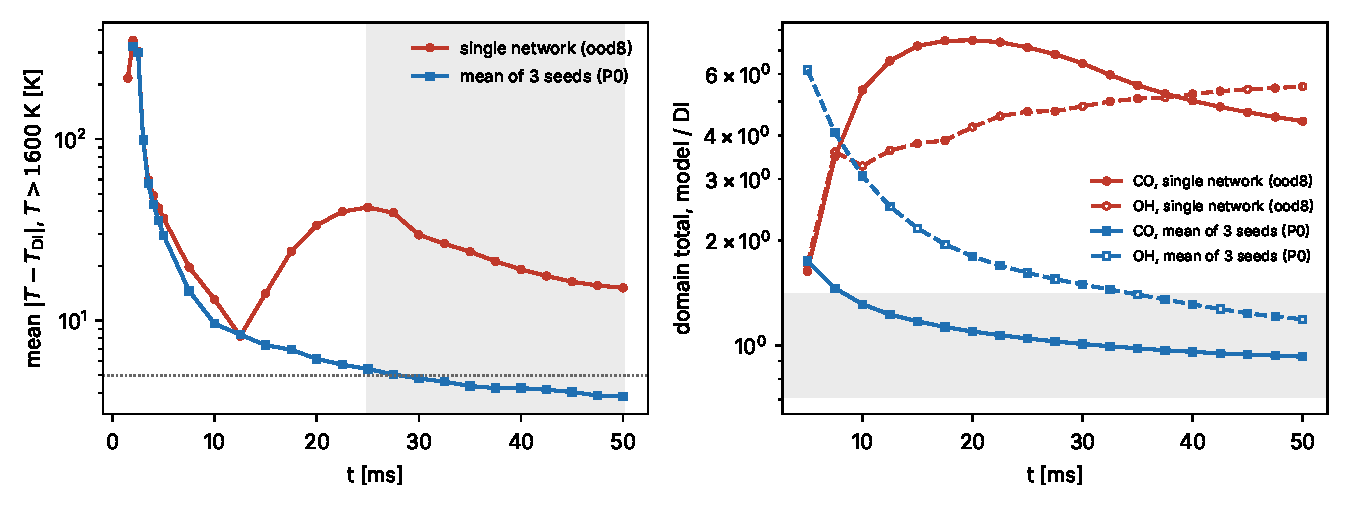
\includegraphics[width=\textwidth]{figs/fig_cfd_flame.pdf}
\caption{Burner simulation in pure mode. Left: mean $|T-T_\mathrm{DI}|$ in the flame zone; the grey band is
the scoring window, the dotted line the 5~K target. Right: domain totals of CO (solid) and OH (dashed)
over those of DI; the grey band is the $\times1.4$ target.}
\label{fig:flame}
\end{figure}

\begin{figure}[t]
\centering
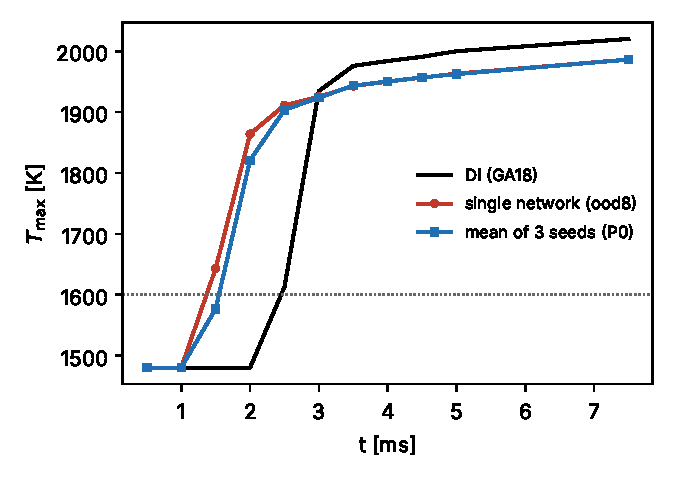
\includegraphics[width=0.6\textwidth]{figs/fig_ignition.pdf}
\caption{Start-up: domain maximum temperature. The dotted line is the 1600~K ignition threshold.}
\label{fig:ign}
\end{figure}

\paragraph{Established flame}
The ensemble meets the flame and species targets that the single network misses by a factor of about
five. Its flame-zone error is 4.4~K against 24.2~K, and does not drift. CO stays within 7\% of DI over the scoring window and OH falls from 1.6 to 1.2 times DI, while ood8
makes 4 to 7 times too much CO and 5 to 6 times too much OH. The
most telling number is the OOD share: with ood8, 58.5\% of the flame cells leave the trained range, and
since pure mode has no fallback, the network keeps advancing them; with the ensemble, 0.4\% do. The
ensemble's smaller one-step errors keep the solution on the states the networks were trained on, and
this compounds over thousands of steps. That is why the gain in the burner (5.5 times in the flame error)
is larger than offline (1.5 to 2.5 times).

\paragraph{Start-up}
Both models ignite the fuel jet early, ood8 by 1.1~ms and the ensemble by 0.9~ms
(Fig.~\ref{fig:ign}); both overshoot the DI maximum temperature during the first 2.5~ms. Since the three
members share their training data and all ignite early, the bias comes from the data (the induction
chemistry of the vitiated and partially burnt states), not from the variance of one network, and
averaging cannot remove it. With this term the ensemble's score is 3.01 against 5.23. For reference, a
single network retrained on physics data seeded at the states where an earlier network failed in this
burner (ITERML iteration 1) scored 2.22 with a 3.3~K flame error \todo{cite}; the ensemble reaches similar
flame and species accuracy from a priori data alone.

\paragraph{Cost}
The ensemble costs 9.84~s per step against 3.42~s, 2.9 times. The chemistry dominates the step, so the
factor is close to the number of members. \todo{Fluent timing on the Windows workstation; the UDF loads
the same ensemble file but has not been compiled and timed yet.}

%% ===============================================================================================
\section{Discussion}
\label{sec:disc}

\paragraph{Why averaging works here}
Networks trained from scratch on the same data make different errors in the regions where data are
thin, and those errors partly cancel in the mean. The spread of results between seeds (25 to 45~K at
10~ms for the same data and architecture) shows that the error of one a priori network is to a large
extent variance, not bias. In a closed loop, removing part of that variance also keeps the trajectory
inside the training data, so the gain compounds. Warm-started seeds share their parent's errors and
give no gain, so the members must be trained independently.

\paragraph{Why partitioning did not pay off yet}
The error map promised a gain from specialisation, but three effects work against it: each expert has
less data; its OOD tables cover only its box, so states near a boundary are flagged more often; and the
one-step increment error grows at the boundaries, where the blend mixes networks that were never trained
to agree. Fine-tuning experts from the single network, the cheapest way to build them, made things worse,
and the same happened to a single network fine-tuned in the same way, which shows that one-step
validation loss is a poor guide to closed-loop accuracy. Partitioning might still pay off with overlapping
training boxes, a consistency loss across the boundaries, or experts that are themselves ensembles.

\paragraph{Disagreement as an OOD signal}
The members' spread predicts the ensemble's error on the benchmark (Spearman up to 0.83 at 1~ms). In a
solver without a fallback, a cell with large spread cannot be sent to DI, but it can be logged and its
state used as a seed of new physics-based exploration, which keeps the training data independent of the
simulation. \todo{Use $\sigma_T$ in the burner: map of the spread against the DI error.}

\paragraph{Cost against accuracy}
A threefold cost buys a fivefold reduction of the flame error and brings CO and OH within target. Whether
that trade is worth it depends on the use: for the pollutant-relevant species it clearly is; for the
temperature field alone, a single network with better data (ITERML) gets there at a third of the cost.
The two are complementary: an ensemble of networks trained on the improved data is the obvious next
test.

\subsection{Limitations}
\label{sec:limits}
\begin{itemize}
\item One burner simulation per model. The ensemble members are fixed, but the single-network baseline
  is the best of three seeds; the other two were not run in the burner, and offline they are twice as
  bad, so the comparison favours the single network.
\item The single network with three times the parameters was not trained, so part of the ensemble's gain
  could be capacity rather than averaging. \todo{Train and run the 3x control if the reviewers ask.}
\item The region experts were not run in the burner.
\item One burner, one mechanism, one architecture, laminar flow.
\item The offline benchmark is not predictive of the burner ranking; it was used only to drop candidates.
\end{itemize}

%% ===============================================================================================
\section{Conclusions}
\label{sec:concl}
\begin{itemize}
\item A deep ensemble of three networks trained from scratch on physics-based data is better than any of
  its members offline, and in a laminar burner simulation without fallback it reduces the flame-zone
  temperature error from 24.2 to 4.4~K, brings the CO and OH totals within the factor-1.4 target on average, and keeps the flame
  inside the trained range, at 2.9 times the cost.
\item Averaging does not correct a bias shared by the members: the early ignition remains, and must be
  fixed in the training data.
\item The spread of the members is a usable uncertainty signal.
\item Region experts with a soft gate on temperature and normalised progress variable were not better than
  single networks by more than the seed noise; experts warm-started from the single network were worse.
\item Seed noise of a priori networks is large (a factor of two in the benchmark error); comparisons of
  single networks should use several seeds.
\end{itemize}

\section*{Data and code availability}
\todo{Repository, model files, ensemble file format (chemmanifold\_ensemble.txt), benchmark states and
protocol reports.}

\section*{Acknowledgements}
\todo{}

\bibliographystyle{elsarticle-num}
\bibliography{refs}

\end{document}
